\documentclass[twocolumn,10pt]{ltjsarticle}

\usepackage[top=15mm,bottom=15mm,left=20mm,right=20mm,columnsep=10mm]{geometry}
\usepackage[haranoaji,nfssonly]{luatexja-preset}
\usepackage{graphicx}
\usepackage{titlesec}
\usepackage{url}

\usepackage{multirow}    % セル結合用
\usepackage{tabularx}    % 表用&カラムサイズ指定

%% カラムサイズの指定用 %%
\newcolumntype{C}[1]{>{\centering\arraybackslash}p{#1}}
\newcolumntype{L}[1]{>{\raggedright\arraybackslash}p{#1}}
\newcolumntype{R}[1]{>{\raggedleft\arraybackslash}p{#1}}

\title{【実験】通信時間の粒度を高めたデータでの周期分析結果}
\author{山下 尚彦}
\date{\today}

\begin{document}
\maketitle

\section{はじめに}
本研究メモは, 正しく通信の周期分析を行えるように, データ処理やプログラムの改善方法の検討と改善後の実験結果, データセットBOS\_2016について報告した論文\cite{weko_175829_1}との比較結果についてまとめる. 

\section{改善方法について}
本章では, 正しく周期分析できなかった原因とその改善方法について検討する.  

\subsection{問題点}
周波数解析によって周期を求める方法は, 高速フーリエ変換や離散フーリエ変換などがあるが, これらはデータのサンプリング間隔が一定であったり, データの数が2のべき乗であったりする必要がある. 一方, Lomb-Scargleピリオドグラムは不定間隔の離散データを周波数解析することができるため, 太陽に現れる黒点の周期を求めるなど, データを同じ時間間隔で取れない天文学や医学, 自動車業界, 通信などに利用される. 

黒点の周期を求める場合, 1日ごとに太陽に黒点が現れたか, または現れなかったかを記録する必要があるが, 前回までの実験では図\ref{fig:e12_result}上部の通信回数と時間の関係を表したグラフのように1秒間に何回通信したかを記録したものをピリオドグラムで解析を行っていた. そのため, 通信観測データから正しく周期性のある通信を検出できなかったと考えられる. 

\begin{figure}[htbp]
    \centering

    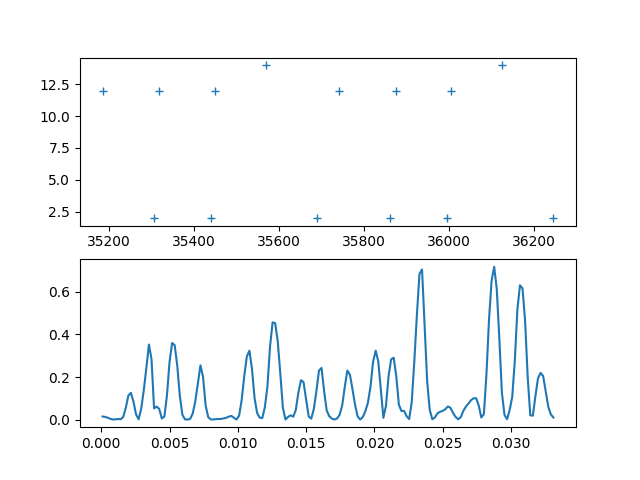
\includegraphics[width=7.5cm]{images/【実験】通信時間の粒度を高めたデータでの周期分析結果/e12.png}

    \caption{e12の通信回数と解析結果}
    \label{fig:e12_result}
\end{figure}

\subsection{データ処理の改善}
本節では2.1節で説明した通信回数と時間関係による問題点の改善を検討する. 

これまで, 通信観測データの処理の際にタイムスタンプをミリ秒以下を切り捨て, YYYY-MM-DDThh:mm:ssの形式でピリオドグラムで周期分析したが, 1秒間に複数回通信を行った場合, 正しい結果が得られない. そこで, タイムスタンプをナノ秒まで使用することで, 図\ref{fig:e12_count}のようにリクエスト/レスポンスのたびにプロットされるようにデータを処理する. 

\begin{figure}[htbp]
    \centering

    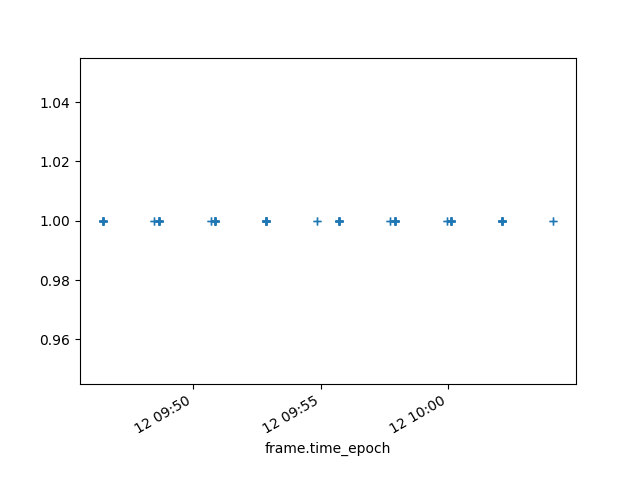
\includegraphics[width=7.5cm]{images/【実験】通信時間の粒度を高めたデータでの周期分析結果/e12_count.png}

    \caption{ナノ秒まで使用した通信回数と通信時間の関係}
    \label{fig:e12_count}
\end{figure}

\subsection{プログラムによる改善}
2.2節で通信発生ごとにデータをプロットすることができたが, Lomb-Scargleピリオドグラムで黒点の周期を求めるように, 通信の周期を分析するためには通信が発生していない場合, 通信回数を0としたデータが必要になる. そこで, 通信発生前後を時間, 分, 秒, ミリ秒, ナノ秒単位でPythonのPandasライブラリによって通信回数0のデータを追加し, 通信が発生した時間と発生していない時間を保持したデータを作成した(図\ref{fig:e12_program}). 

\begin{figure}[htbp]
    \centering

    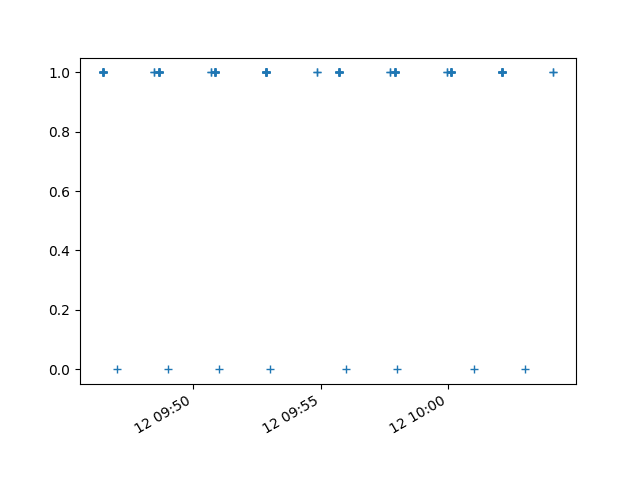
\includegraphics[width=7.5cm]{images/【実験】通信時間の粒度を高めたデータでの周期分析結果/e12_program.png}

    \caption{通信回数0を追加した通信回数と通信時間の関係}
    \label{fig:e12_program}
\end{figure}

\section{結果}
本章では, 通信観測データの周期分析実験の結果について述べる. なお, 本研究メモではマルウェア検体が動作しC2サーバとのTCPコネクションを確立したが, HTTPのステータスコードが403(Forbidden),404(Not Found), 503(Service Unavailable)などでC2サーバとの通信が成立しなかったe12とe20と, マルウェアが活動しTCP SYNパケットをC2サーバに送信したが, TCPコネクションを確立できなかったe70, e435の解析結果について記述する. 

表\ref{tab:e12}, \ref{tab:e20}, \ref{tab:e70}, \ref{tab:e435}は, e12とe20, e70, e435の通信観測データを1日ごとに解析し, 送信元IP数(SRC), 送信元と受信先IPペア数(PAIR), 周期的である確率が99.9\%以上ある通信を行ったIPアドレスのペア数をまとめた表である. 

\begin{table}[htbp]
    \centering
    \caption{e12の実験結果}

    \begin{tabular}{c||lll}
        %% カラム名 %%
        \hline
        DATE & SRC & PAIR & 99.9\% \\
        \hline \hline
        %% データ %%
        20160212  & 21 & 42 & 9 \\
        20160213  & 5  & 8  & 0 \\
        20160215  & 8  & 14 & 7 \\
        20160216  & 4  & 6  & 0 \\
        \hline
    \end{tabular}

    \label{tab:e12}
\end{table}

\begin{table}[htbp]
    \centering
    \caption{e20の実験結果}

    \begin{tabular}{c||lll}
        %% カラム名 %%
        \hline
        DATE & SRC & PAIR & 99.9\% \\
        \hline \hline
        %% データ %%
        20160215  & 14 & 27 & 3 \\
        20160216  & 5  & 8  & 1 \\
        20160217  & 5  & 8  & 1 \\
        20160218  & 8  & 15 & 7 \\
        \hline
    \end{tabular}

    \label{tab:e20}
\end{table}

\begin{table}[htbp]
    \centering
    \caption{e70の実験結果}

    \begin{tabular}{c||lll}
        %% カラム名 %%
        \hline
        DATE & SRC & PAIR & 99.9\% \\
        \hline \hline
        %% データ %%
        20160215  & 16 & 34 & 14 \\
        20160216  & 7  & 15 & 11 \\
        20160217  & 12 & 25 & 11 \\
        20160218  & 7  & 16 & 12 \\
        \hline
    \end{tabular}

    \label{tab:e70}
\end{table}

\begin{table}[htbp]
    \centering
    \caption{e435の実験結果}

    \begin{tabular}{c||lll}
        %% カラム名 %%
        \hline
        DATE & SRC & PAIR & 99.9\% \\
        \hline \hline
        %% データ %%
        20160328 & 16 & 31 & 2 \\
        20160329 & 2  & 3  & 1 \\
        20160330 & 5  & 9  & 2 \\
        \hline
    \end{tabular}

    \label{tab:e435}
\end{table}

\subsection{Case e12}
e12はC2サーバとTCPコネクションを確立できたが, C2サーバとの通信が成立しなかった事例で, C2サーバのIPアドレスは\ast\ast\ast.56.81.119と\ast\ast\ast.76.86.155である. 表\ref{tab:e12_ip}から2016年2月12日にC2サーバのIPアドレスを両方とも検出することができた. 図\ref{fig:e12_result1}は\ast\ast\ast.56.81.119との通信回数とLomb-Scargleピリオドグラムによる解析結果を表した図で, 同様に図\ref{fig:e12_result2}は\ast\ast\ast.76.86.155の図である. 

\begin{table}[htbp]
    \centering
    \caption{e12で周期的な通信を示した受信先IP}

    \begin{tabular}{|c||c|l|}
        \hline
        DATE & PERIODIC & IP ADDRESS \\
        \hline \hline
        20160212 & 99.9\% & \begin{tabular}{l}
                               \ast\ast\ast.79.197.250 \\
                               \ast\ast\ast.32.241.24  \\
                               \ast\ast\ast.56.81.119  \\
                               \ast\ast\ast.76.86.155
                            \end{tabular} \\ \hline
        20160215 & 99.9\% & \begin{tabular}{l}
                               \ast\ast\ast.76.4.147   \\
                               \ast\ast\ast.59.139.27  \\
                               \ast\ast\ast.59.160.60  \\
                               \ast\ast\ast.213.168.19
                            \end{tabular} \\ \hline
    \end{tabular}

    \label{tab:e12_ip}
\end{table}

\begin{figure}[htbp]
    \centering

    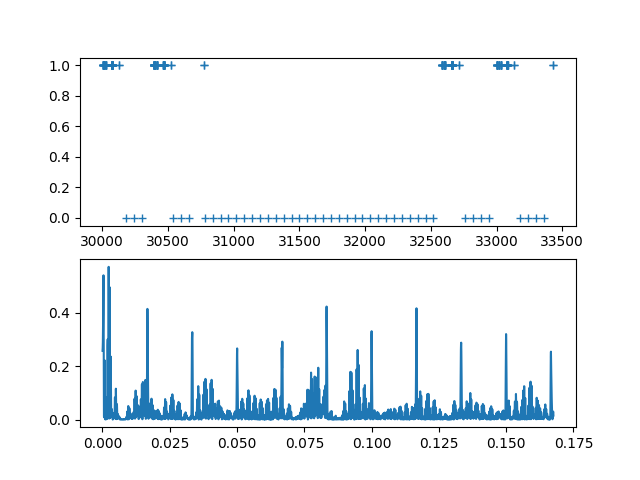
\includegraphics[width=7.5cm]{images/【実験】通信時間の粒度を高めたデータでの周期分析結果/e12/c2-1.png}

    \caption{\ast\ast\ast.56.81.119の通信回数と解析結果}
    \label{fig:e12_result1}
\end{figure}

\begin{figure}[htbp]
    \centering

    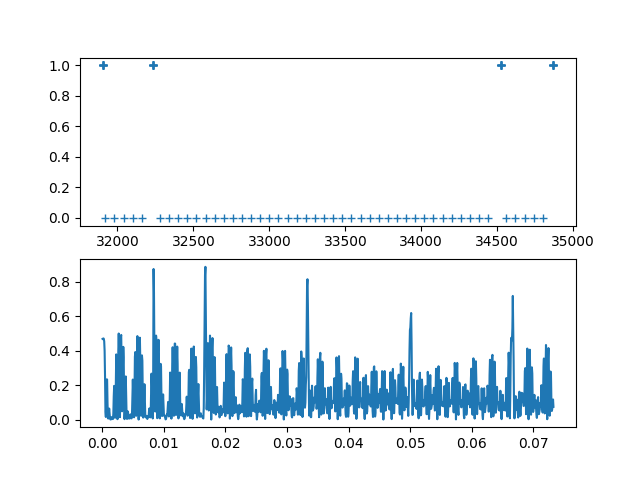
\includegraphics[width=7.5cm]{images/【実験】通信時間の粒度を高めたデータでの周期分析結果/e12/c2-2.png}

    \caption{\ast\ast\ast.76.86.155の通信回数と解析結果}
    \label{fig:e12_result2}
\end{figure}

\subsection{Case e20}
e20もe12と同様に, C2サーバとTCPコネクションを確立できたが通信が成立しなかった事例である. e20のC2サーバのIPアドレスは\ast\ast\ast.81.81.137である. しかし表\ref{tab:e20_ip}から分かるように, 今回の実験ではC2サーバとの周期的な通信を検出できなかった. 

\begin{table}[htbp]
    \centering
    \caption{e20で周期的な通信を示した受信先IP}

    \begin{tabular}{|c||c|l|}
        \hline
        DATE & PERIODIC & IP ADDRESS \\
        \hline \hline
        20160215 & 99.9\% & \begin{tabular}{l}
                               \ast\ast\ast.32.1.160   \\
                               \ast\ast\ast.107.4.50   \\
                               \ast\ast\ast.58.221.163
                            \end{tabular} \\ \hline
        20160216 & 99.9\% & \begin{tabular}{l}
                               \ast\ast\ast.118.6.83
                            \end{tabular} \\ \hline
        20160218 & 99.9\% & \begin{tabular}{l}
                               \ast\ast\ast.32.1.160   \\
                               \ast\ast\ast.36.102.106 \\
                               \ast\ast\ast.113.237.189
                            \end{tabular} \\ \hline
    \end{tabular}

    \label{tab:e20_ip}
\end{table}

\subsection{Case e70, e435}
マルウェアが動作したがTCPコネクションを確立できなかったe70とe435のそれぞれのC2サーバのIPアドレスは, \ast\ast\ast.106.20.192と\ast\ast\ast.24.93.253である. 表\ref{tab:e70_ip}と表\ref{tab:e435_ip}から実験によってC2サーバの周期的な通信を検出できたことが分かる. 

\begin{table}[htbp]
    \centering
    \caption{e70で周期的な通信を示した受信先IP}

    \begin{tabular}{|c||c|l|}
        \hline
        DATE & PERIODIC & IP ADDRESS \\
        \hline \hline
        20160215 & 99.9\% & \begin{tabular}{l}
                               \ast\ast\ast.32.101.160  \\
                               \ast\ast\ast.165.83.176  \\
                               \ast\ast\ast.21.181.152  \\
                               \ast\ast\ast.208.153.9   \\
                               \ast\ast\ast.106.149.145 \\
                               \ast\ast\ast.106.20.192  \\
                               \ast\ast\ast.106.253.18
                            \end{tabular} \\ \hline
        20160216 & 99.9\% & \begin{tabular}{l}
                               \ast\ast\ast.32.101.160  \\
                               \ast\ast\ast.165.83.176  \\
                               \ast\ast\ast.21.181.152  \\
                               \ast\ast\ast.208.153.9   \\
                               \ast\ast\ast.106.149.145 \\
                               \ast\ast\ast.106.20.192  \\
                               \ast\ast\ast.106.253.18
                            \end{tabular} \\ \hline
        20160217 & 99.9\% & \begin{tabular}{l}
                               \ast\ast\ast.32.101.160  \\
                               \ast\ast\ast.165.83.176  \\
                               \ast\ast\ast.21.181.152  \\
                               \ast\ast\ast.208.153.9   \\
                               \ast\ast\ast.106.149.145 \\
                               \ast\ast\ast.106.20.192  \\
                               \ast\ast\ast.106.253.18
                            \end{tabular} \\ \hline
        20160218 & 99.9\% & \begin{tabular}{l}
                               \ast\ast\ast.32.101.160  \\
                               \ast\ast\ast.165.83.176  \\
                               \ast\ast\ast.21.181.152  \\
                               \ast\ast\ast.208.153.9   \\
                               \ast\ast\ast.106.149.145 \\
                               \ast\ast\ast.106.20.192  \\
                               \ast\ast\ast.106.253.18
                            \end{tabular} \\ \hline
    \end{tabular}

    \label{tab:e70_ip}
\end{table}

\begin{table}[htbp]
    \centering
    \caption{e435で周期的な通信を示した受信先IP}

    \begin{tabular}{|c||c|l|}
        \hline
        DATE & PERIODIC & IP ADDRESS \\
        \hline \hline
        20160328 & 99.9\% & \begin{tabular}{l}
                               \ast\ast\ast.24.93.253  \\
                               \ast\ast\ast.213.168.10
                            \end{tabular} \\ \hline
        20160329 & 99.9\% & \begin{tabular}{l}
                               \ast\ast\ast.24.93.253
                            \end{tabular} \\ \hline
        20160330 & 99.9\% & \begin{tabular}{l}
                               \ast\ast\ast.24.93.253
                            \end{tabular} \\ \hline
    \end{tabular}

    \label{tab:e435_ip}
\end{table}

\begin{figure}[htbp]
    \centering

    \includegraphics[width=7.5cm]{images/【実験】通信時間の粒度を高めたデータでの周期分析結果/e70/c2.png}

    \caption{\ast\ast\ast.106.20.192の通信回数と解析結果}
    \label{fig:e70_result}
\end{figure}

\begin{figure}[htbp]
    \centering

    \includegraphics[width=7.5cm]{images/【実験】通信時間の粒度を高めたデータでの周期分析結果/e435/c2.png}

    \caption{\ast\ast\ast.24.93.253の通信回数と解析結果}
    \label{fig:e435_result}
\end{figure}

\section{考察}
本章では, 実験の結果から考察を行う. 

今回の実験では, C2サーバとTCPコネクションを確立できたが通信が成立しなかったe12, e20とC2サーバとのTCPコネクションが確立できず, TCP SYNパケットを送信し続けたe70, e435の通信観測データをLomb-Scargleピリオドグラムによって解析した. 実験の結果, e12とe70, e435でC2サーバとの周期的な通信を検出できたが, e20では検出した周期的な通信の中にC2サーバとの通信が含まれていなかった. これは図\ref{fig:e20_count}から分かるように, 短時間に3回しか通信を行っていないことが原因と考えられる. 

また, 表\ref{tab:e12}から\ref{tab:e435}のそれぞれの事例で周期的な通信を行った数に着目すると, 送信元と受信先のIPアドレスのペア数と比べて, それほど絞り込むことができないように見える. これは, マルウェアの通信以外に周期的な通信を行っていたプログラムやソフトウェアがあったためと思われる. 既存の手法を組み合わせることで, C2サーバとの通信をより高精度に検出することができると考えられる. 

\begin{figure}[htbp]
    \centering

    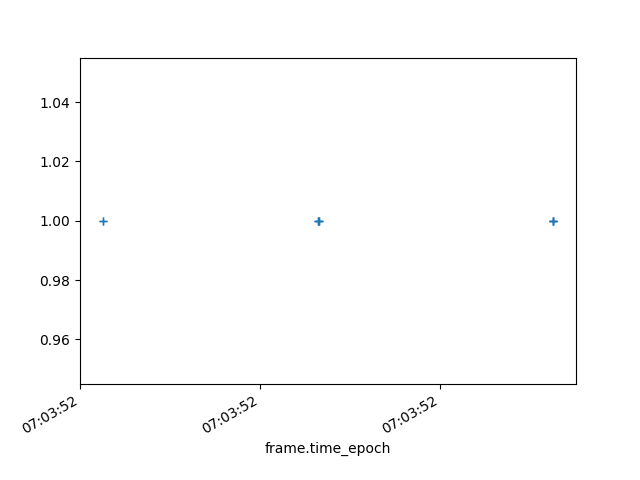
\includegraphics[width=7.5cm]{images/【実験】通信時間の粒度を高めたデータでの周期分析結果/e20/count.png}

    \caption{\ast\ast\ast.81.81.137の通信回数}
    \label{fig:e20_count}
\end{figure}

\section{おわりに}
本研究メモでは, これまでのデータ処理やプログラムを修正して, C2サーバの通信を検出できなかった問題を改善する方法を検討し, 実際に修正して実験を行った結果と考察について述べた. 

Lomb-Scargleピリオドグラムによる解析の結果, e12, e70, e435でC2サーバとの周期的な通信を検出することができた. しかし, 検出した周期的な通信が比較的存在したため既存の手法と組み合わせることで, より精度の高い検出を試みたい. 一方で, e20のように短時間に数回のみC2サーバと通信した事例ではLomb-Scargleピリオドグラムによる検出は困難であった. 

\bibliographystyle{junsrt}
\bibliography{DB}
\end{document}